\documentclass[department=icis, notes={show notes}, slidesperpage=1, official=true,showdate=true,slidenumbers=relative]{beamerruhuisstijl}

\usepackage[british]{babel}
\usepackage{graphicx,hyperref,url}
\usepackage{amsmath,amssymb,amsfonts}
\usepackage{listings}  
\usepackage{enumitem}
\usepackage{courier}

\setitemize{noitemsep,topsep=0pt,parsep=0pt,partopsep=0pt,itemsep=1pt,label=$\bullet$}
\lstset{language=clean,showstringspaces=false,basicstyle=\footnotesize\ttfamily}


\newcommand{\projecttitle}{Developing Real Life, Task Oriented Applications for the Internet of Things}
\newcommand{\rinus}{prof.~dr.~dr.h.c.~ir.~M.J.~Plasmeijer }
\newcommand{\pieter}{dr.~P.W.M. Koopman}
\newcommand{\mart}{M. Lubbers MSc.}

\author{Matheus Amazonas Cabral de Andrade}
\title[]{\projecttitle}
\subtitle{Master's Thesis Presentation}
\institute[Radboud University Nijmegen]{Institute for Computing and Information Sciences \\
  Radboud University Nijmegen}
\date{\today}


\begin{document}

\begin{frame}[plain]
  \titlepage
\end{frame}

\begin{frame}[fragile]
    \frametitle{Master's Thesis}
    \begin{itemize}
        \setlength\itemsep{1em}
        \item Master's in Computing Science (Software Science)
        \item iCIS's Software Science Department
        \item Project Supervisor: \rinus
        \item Daily Supervisor: \mart
        \item Second Reader: \pieter
    \end{itemize}
\end{frame}

\section{Introduction}
\begin{frame}[fragile]
  \frametitle{Introduction}
    \begin{itemize}
        \setlength\itemsep{1em}
        \item{Task-Oriented Programming (TOP)}
        \begin{itemize}[label=$\diamond$]
            \item High level of abstraction
            \item Clean implementation: iTasks
            \item Many platforms
        \end{itemize}
        \item{Internet of Things (IoT)}
        \begin{itemize}[label=$\diamond$]
            \item Microcontrollers
            \item Internet
            \item Ubiquitous
            \item But no TOP
        \end{itemize}
    \end{itemize}
\end{frame}


\section{mTask}
\begin{frame}[fragile]
  \frametitle{mTask}
  \begin{itemize}
      \setlength\itemsep{1em}
      \item Embedded Domain Specific Language
      \item Motivation
      \item Two views
      \begin{itemize}[label=$\diamond$]
          \item Code
          \item Interpret
      \end{itemize}
      \item The Interpreted View
      \begin{itemize}[label=$\diamond$]
          \item Motivation
          \item Client
          \item Simulator
      \end{itemize}
  \end{itemize}
\end{frame}

\section{Example}
\begin{frame}[fragile,c]
  \frametitle{mTask Example: Factorial}
  \begin{lstlisting}
factorial :: (Shared Int) Int -> Main (ByteCode () Stmt)
factorial si i = sds \y=i In lowerSds \x=si In {main =
    IF (y <=. lit 1) (
		pub x :. 
		ledOn (lit LED1) :.
		retrn
	) (
		x =. x *. y :.
		y =. y -. lit 1
	)}
    \end{lstlisting}
\end{frame}

\section{Research Question}
\begin{frame}[plain,c]
    \frametitle{Research Question}
    \begin{center}
        Is it possible to develop real-life, IoT applications using mTask? If so, how can the development process be improved? If not, what are the challenges to solve to make it possible?
    \end{center}
\end{frame}

\section{Application Domain}
\begin{frame}[fragile]
    \frametitle{Application Domain}
    \begin{itemize}
        \setlength\itemsep{1em}
        \item Selection Criteria
        \item Home Automation
        \item Autohouse
        \begin{itemize}[label=$\diamond$]
            \item Architecture
            \item Tasks
            \item Devices
        \end{itemize}
    \end{itemize}
\end{frame}

\section{Development}
\begin{frame}[fragile]
    \frametitle{Development Overview}
    \begin{itemize}
        \item Simulator on early stages of development
        \item Wireless communication
        \item Device deployment
    \end{itemize}
\end{frame}

\begin{frame}[fragile,c]
    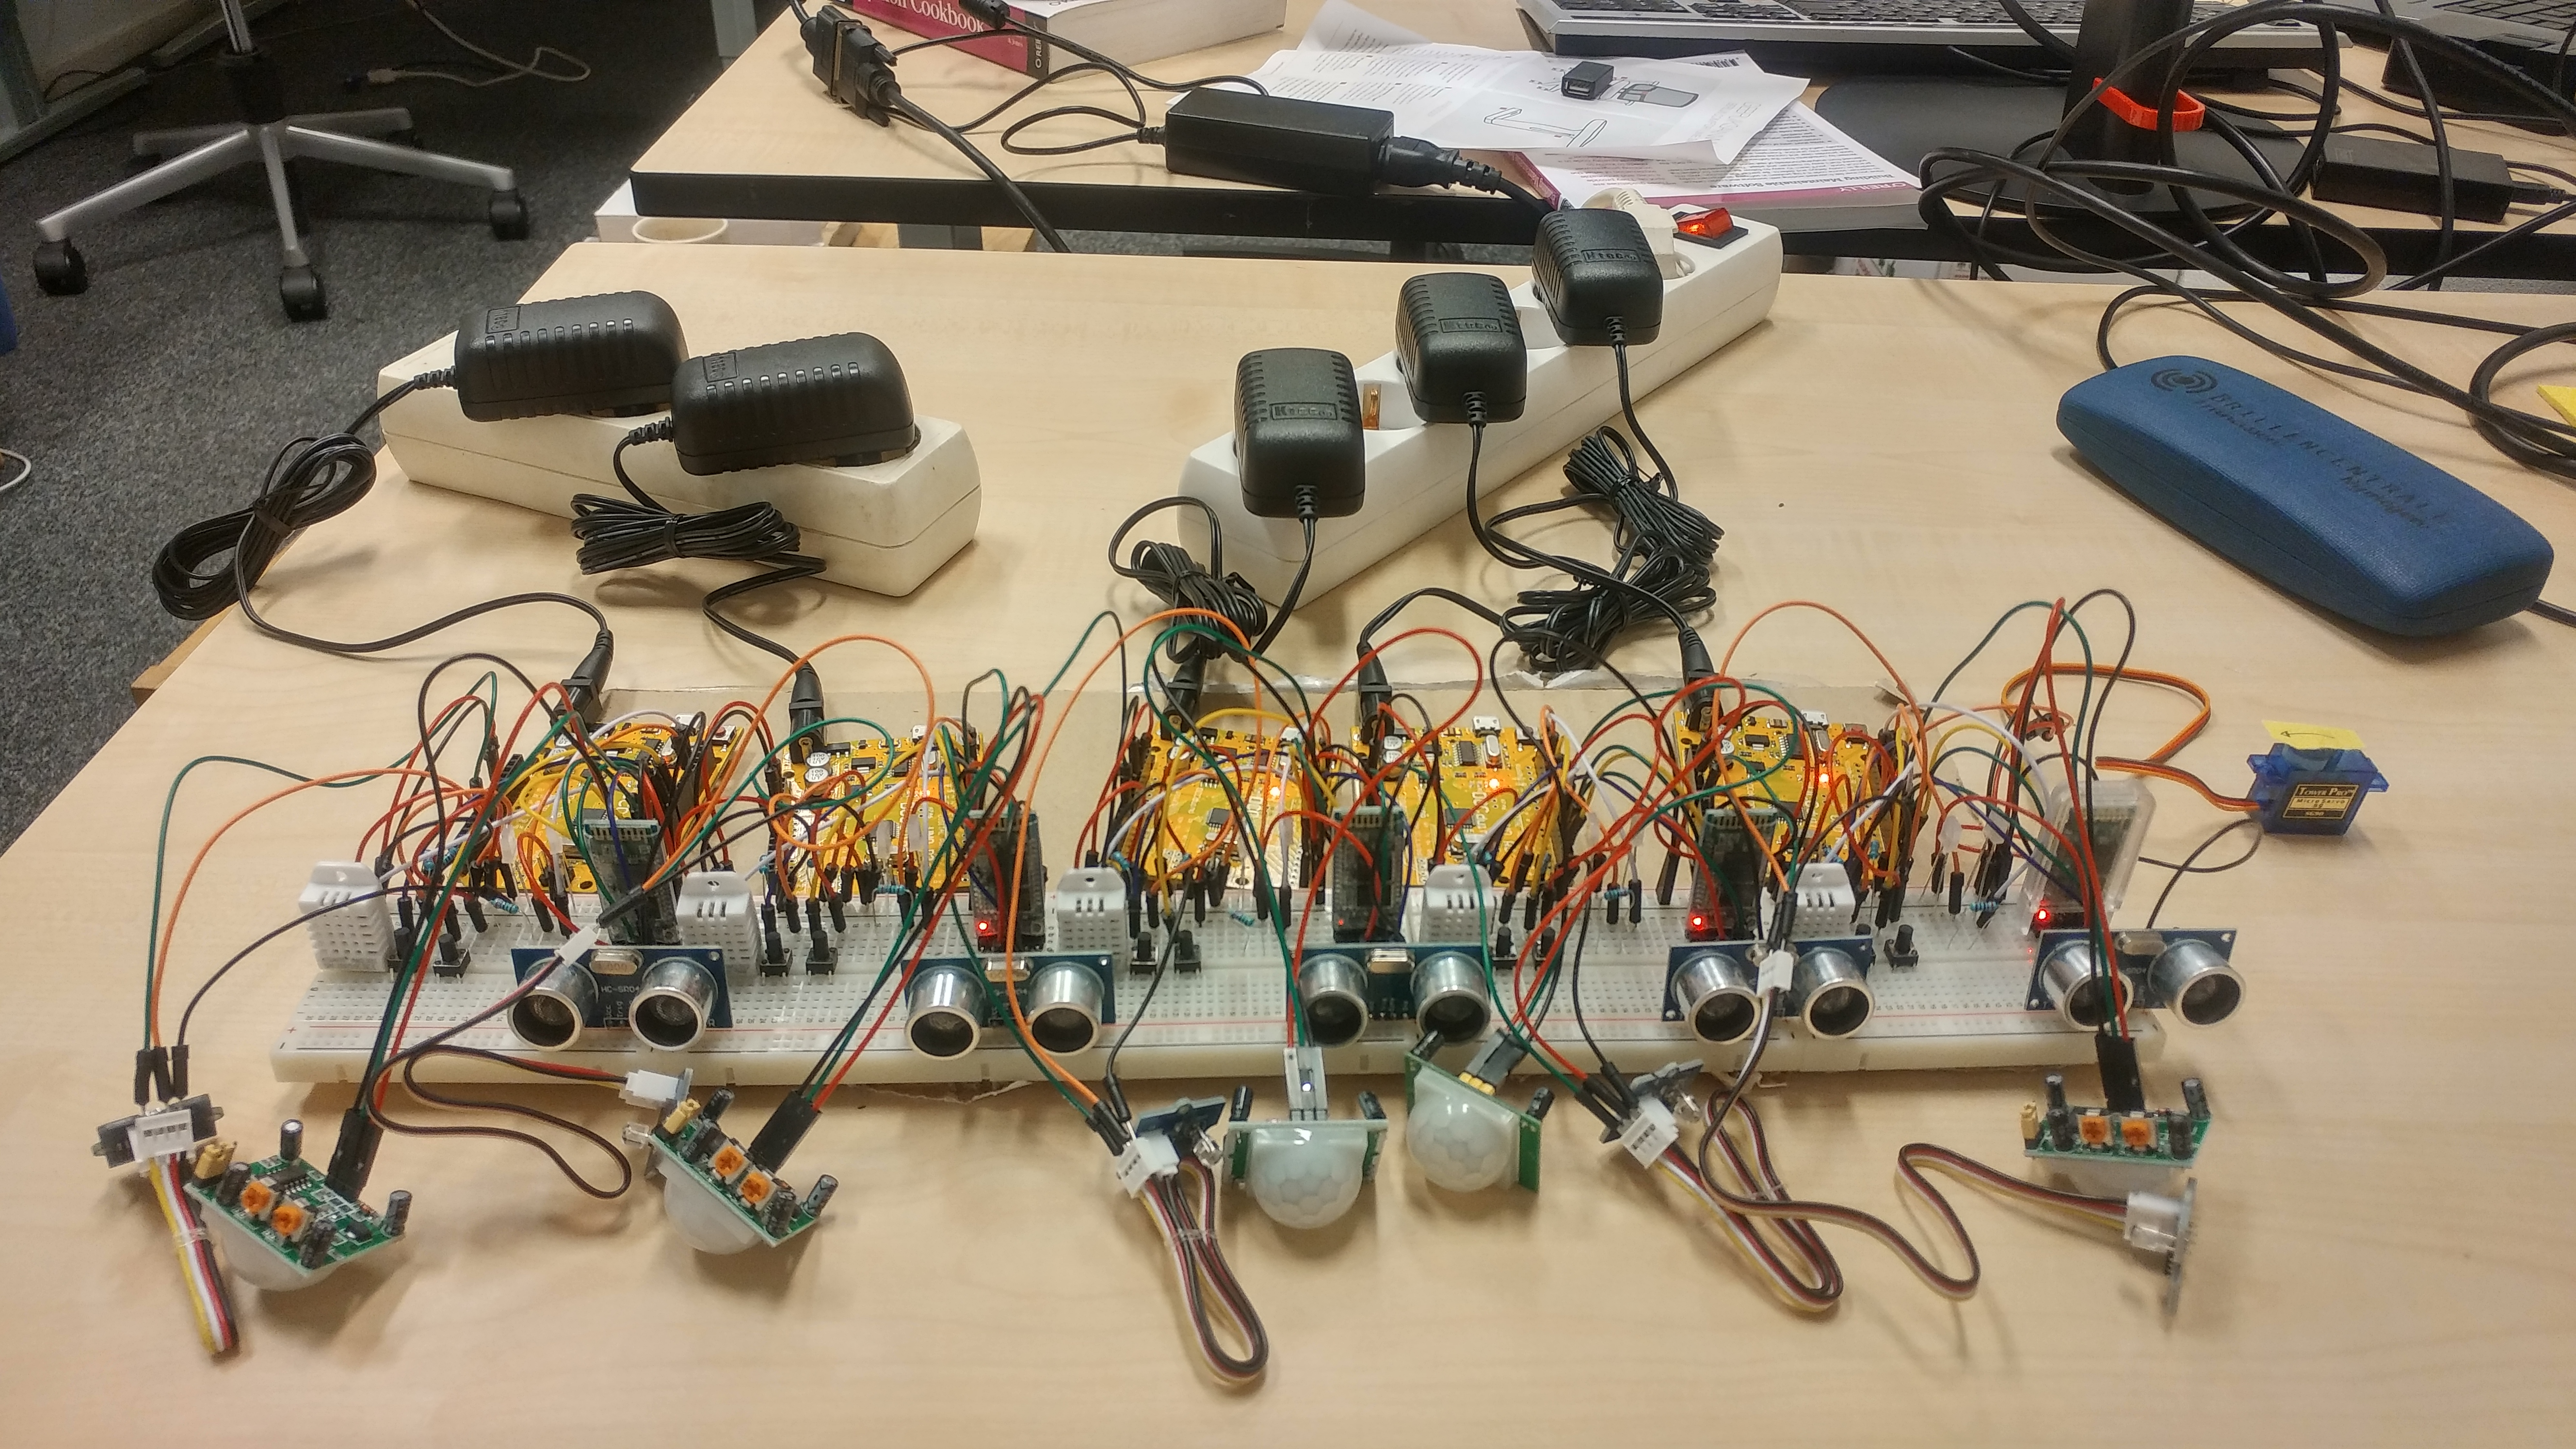
\includegraphics[scale=0.06]{presentation/img/side.jpg}
\end{frame}

\begin{frame}[fragile,c]
    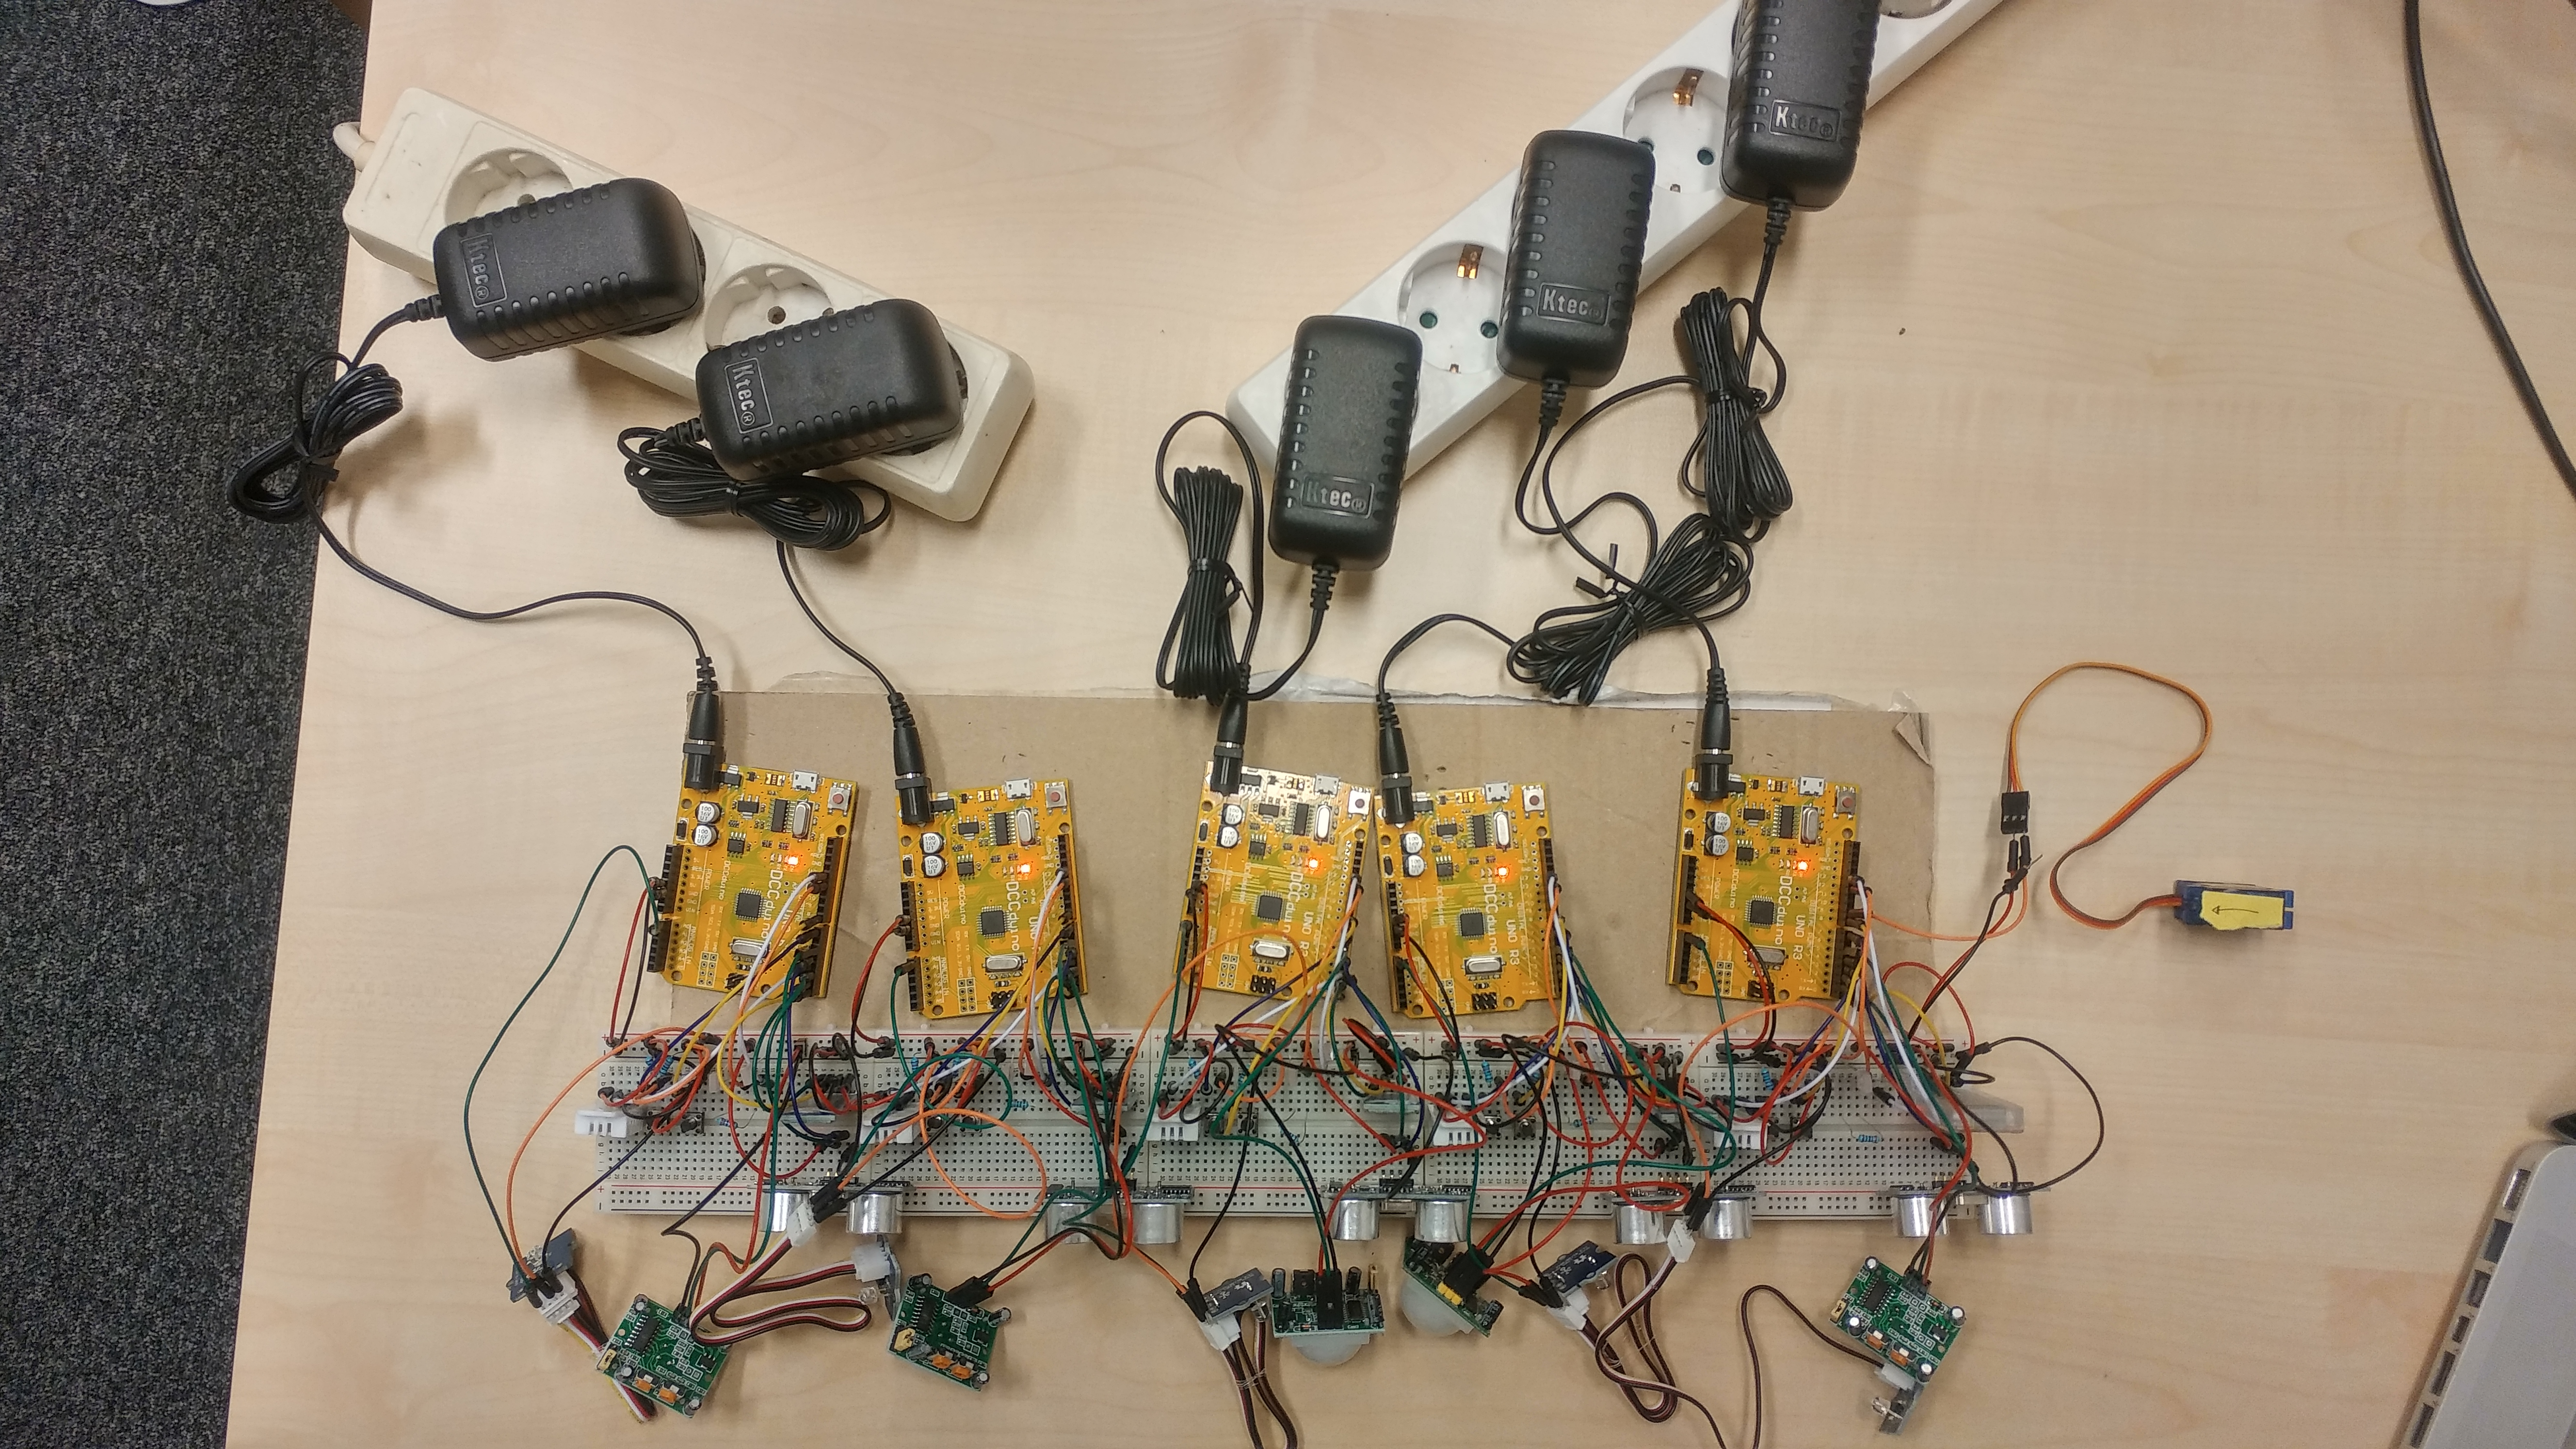
\includegraphics[scale=0.06]{presentation/img/top.jpg}
\end{frame}


\begin{frame}[fragile]
    \frametitle{Changes to mTask}
    \begin{itemize}
        \setlength\itemsep{1em}
        \item Variables
        \item New peripherals
        \item Requirements view
        \item Device disconnection
        \item Simulator improvements
    \end{itemize}
\end{frame}

\begin{frame}[fragile]
    \frametitle{Limitations of mTask}
    \begin{itemize}
        \setlength\itemsep{1em}
        \item SDSs live forever
        \item Unwanted SDS update loop
        \item No task acknowledgment communication
        \item Floating-point arithmetic
    \end{itemize}
\end{frame}

\begin{frame}[fragile]
    \frametitle{Task Migration}
    \begin{itemize}
        \setlength\itemsep{1em}
        \item Device disconnection recogniziton
        \begin{itemize}[label=$\diamond$]
            \item Using the connection error handler
        \end{itemize}
        \item Migration strategies
        \begin{itemize}[label=$\diamond$]
            \item Do not migrate
            \item Same room
            \item Any room
        \end{itemize}
        \item Migration to compatible devices
        \begin{itemize}[label=$\diamond$]
            \item Using the Requirements view
        \end{itemize}
    \end{itemize}
\end{frame}

\section{Demo}
\begin{frame}[plain,c]
  \frametitle{}
  \begin{center}
    \Huge Demo
  \end{center}
\end{frame}

\section{Conclusion}
\begin{frame}[fragile]
  \frametitle{Conclusion}
  \begin{itemize}
      \setlength\itemsep{1em}
      \item A real-life application was developed using mTask
      \item mTask was improved
        \begin{itemize}[label=$\diamond$]
            \item Changes to mTask
        \end{itemize}
      \item Future work on mTask
        \begin{itemize}[label=$\diamond$]
            \item Overcome the limitations found during research
            \item mTask2
            \item Test mTask performance
            \item Test mTask with the Raspberry Pi
        \end{itemize}
      \item Future work on Autohouse
        \begin{itemize}
            \item Task migration with tags
            \item Peripheral sharing
        \end{itemize}
  \end{itemize}
\end{frame}

\begin{frame}[plain,c]
  \frametitle{}
  \begin{center}
    \Huge Questions?
  \end{center}
\end{frame}


\begin{frame}[plain,c]
  \frametitle{}
  \begin{center}
    \Huge Thank you
  \end{center}
\end{frame}

\end{document}
